\section{Modeling}
\label{sec:modeling}


% %
% SYSTEM DESCRIPTION
% %
Mobile devices are still limited in computing capabilities and battery lifetime. The problem of enhancing user
experience may find a solution in cloud computing.
Consider a "two-layer" cloud system, consisting of an edge cloud server (cloudlet) and a remote cloud server, where
the cloudlet is at "one-hop" distance from a set of mobile devices. Applications running on these mobile devices
autonomously select some of their tasks for offloading to an external server (e.g., because of performance or energy
saving reasons), and send an offloading request to a controller located on the cloudlet. Upon receiving a request, the
controller takes a decision about whether the task should be sent to the cloudlet or the cloud, with the goal of
minimizing the mean response time.
Typically, tasks hosted by the cloud server benefit of a higher execution rate, but suffer for greater network delay.
We assume that the remote cloud server has virtually unlimited resources, hence it is always able to guarantee
absence of interference among any number of tasks allocated to it. On the other hand, the cloudlet has limited
resources, so that it is able to guarantee absence of interferences among tasks allocated to it as long as their number
does not exceed a given threshold N.
%
Consider the following modeling assumptions:
• The users belong to two classes, class 1 and class 2, with the following arrival rates:
lambda 1 = 3.25 task/s, lambda 2 = 6.25 task/s
• The service both on cloudlet and on the cloud can be assumed exponential, with the following rates:
mu 1clet = 0.45 task/s, mu 1cloud = 0.25 task/s
mu 2clet = 0.30 task/s, mu 2cloud = 0.22 task/s
Note that, as we stated above, the service time includes the transmission time. We assume mu iclet > mu icloud for both
classes. Moreover, note that the execution on the cloudlet of a class 1 task is more convenient than the execution of a
class 2 task.
Let us denote with (n 1 , n 2 ) the state of the system, with n i the number of class i tasks in execution on the cloudlet, and
with S <= N a given threshold. Under the above assumptions, the controller can take the following decisions upon task
arrival events:
%
class 1arrival:
if n1=N ! send on the cloud
else if n1+n2<S ! accept
else if n2 > 0 ! accept the task on the cloudlet and send a class 2 task on the cloud
else accept the task on the cloudlet
class 2 arrival:
if n1+n2>=S ! send on the cloud
else accept the task on the cloudlet
%
When a class 2 task is interrupted and sent on the cloud, a setup time s setup has to be considered to restart the task on
the cloud. We assume an exponential time with mean E[s setup ]= 0.8 s.
Define a queuing model for the system above.
2. Simulate the system model with N=20 and evaluate the system response time and the effective 1 throughput
as a function of the threshold S.
a. Determine if the system is stationary or not and design the experiments accordingly.
b. For a S=N estimate the distribution of the response time. Motivate the chosen methodology and
conjecture about the shape in respect to known distributions.
3. Determine a threshold S to minimize the response time. Hints: you can start with S=N and try 2 different
values for S
The steady state or transient statistics should be computed with a 95\% confidence level.


% %
% GOALS AND OBJECTIVES
% %
\lipsum[1]


% %
% CONCEPTUAL MODEL
% %
\lipsum[1]

\begin{figure}
  \label{fig:conceptual-model}
  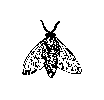
\includegraphics{fig/fly}
  \caption{The conceptual model.}
\end{figure}

% %
% SPECIFICATION MODEL
% %
\lipsum[1]

% %
% VERIFICATION
% %
\lipsum[1]

% %
% VALIDATION
% %
\lipsum[1]
